\newcommand{\ImgLevelBasedTesting}[1]{
    \begin{figure}[h!]
    	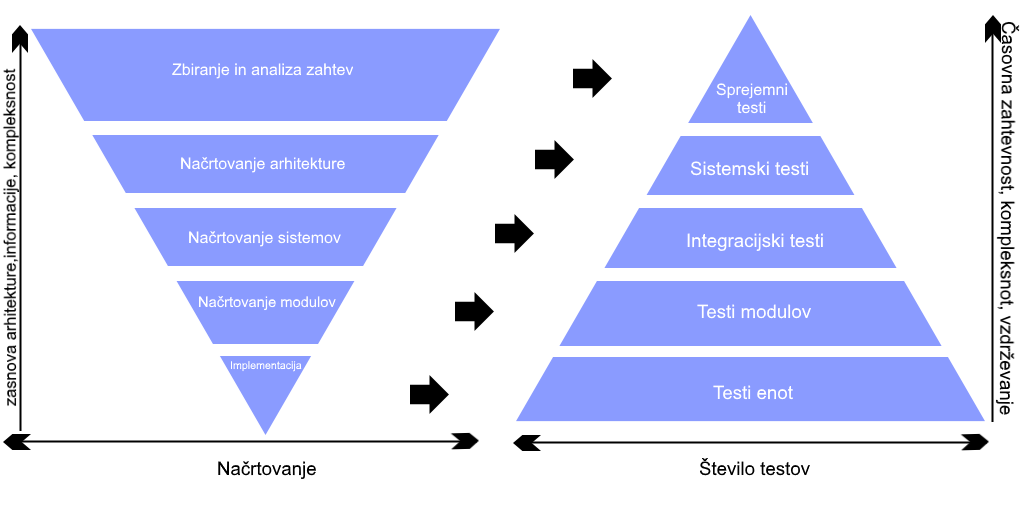
\includegraphics[scale=#1]{img/automation_tests/GrafTestiranja.png}
    	\caption{Stopnje testiranja glede na dejavnost v razvoju}
        \label{fig:LevelBasedTesting}
    \end{figure}
}

\chapter{Avtomatski test}

\section{Stopnje testiranja glede na dejavnost v razvoju}
Avtomatski teste lahko pogrupiramo v različlne skupine glede na dejavnost v razvoju~\cite{Ammann:2008:IST:1355340}. Te dejavnosti so:
\begin{itemize}
    \item Zbiranje in analiza specifikacij in zahtev od klienta ali uporabnik. Za to moramo ustvariti \textbf{sprejemne teste} (ang. Acceptance tests), ki bodo preverjali ali naš program zadošča uporabnikovih potrebam in zahtevam. Ponavadi te teste izvaja končni uporabnik ali nekdo z domenskim znanjem.
    \item Načrtovanje arhitekture projekta/programa. Testom, ki bodo testirali ta del programa pravimo \textbf{sistemski testi} (ang. System tests). Njihova primarna naloga je preveriti ali produkt kot enota deluje pravilno ter če vsi sistemi med seboj pravilno delujejo in komunicirajo. Te testi predvidevajo, da sistemi sami po sebi delujejo pravilno.
    \item Načrtovanje sistemov. Vsak sistem je sestavljen iz več modulov in z \textbf{integracijskimi testi}(ang. Integration tests) preverimo ali te moduli med sabo pravilno komunicirajo in če imajo pravilne informacije drug o drugem.
    \item Načrtovanje modulov. \textbf{Testi modulov}(ang. Module testing) preverjajo vsak modul v izolaciji od drugega. Vsak modul je sestavljen iz manjših enot(lahko bi tudi rekli funkcij). Modulom v nekaterih jezikih rečemo kar razredi (ang. classes) ali paketi (ang. packages). Bolj natančno te testi preverjajo kako delujejo enote med sabo.
    \item Implementacija enot. \textbf{Testi enot} so najnižja raven testiranja in ti preverjajo implementacijo enot in kaj neka enota vrne glede na dani vhod. 
\end{itemize}
So tudi prikazane v spodnji \ref{fig:LevelBasedTesting}

V diplomski nalogi se bom osredotočil na teste enot, integracijske teste in sistemske teste, saj je to ponavadi v praksi naloga razvijalcev. 


\ImgLevelBasedTesting{0.5}


TODO:
\begin{itemize}
    \item Unit tests~\cite{sandi_pangerc}~\cite{gorazd_kovacic}
    \item Integration tests~\cite{sandi_pangerc}~\cite{gorazd_kovacic}
    \item napisati unit teste in integracijske teste za mojo igro~\cite{unity_test_runner}~\cite{nunit}
    \item raziskati test driven development
    \item povezati behavior driven development z strojnim učenjem in umetno inteligenco
    \item primerjava avtomatskih testov z ročnim testiranjem in strojnim učenjem
\end{itemize}